\section{}(10 points)
\textbf{Estimate the gravitational bounding energy of a white dwarf and compare this energy to that of a neutron star. Would the energy released from the nuclear burning of a 1.4 $M_\odot$ Carbon white dwarf unbound it? Could the energy unbound a neutron star
of a similar mass?}

The gravitational potential is given by
\begin{equation*}
    \Omega = \frac{3}{5-n}\frac{GM^2}{R}
\end{equation*}
where $n$ is the polytrope index. For both the neutron star and a white dwarf, the polytrope index is $n=3$  which corresponds to a relativistic degenerate gas. Given a mass of $1.4M_\odot$, the gravitational potential for a white dwarf and a neutron star will be 
\begin{equation*}
    \Omega_{WD}=\frac{3}{2}\frac{G(1.4M_\odot)^2}{R_{WD}}=\SI{1.22e+51}{\erg} \quad\text{and}\quad \Omega_{NS}=\frac{3}{2}\frac{G(1.4M_\odot)^2}{R_{NS}} =\SI{7.77e+55}{\erg} , \text{ respectively.}
\end{equation*}
considering that the white dwarf has $R_{WD}\sim R_\oplus$ and a neutron star has $R_{NS} \sim \SI{10}{\km}$, obtained from Fig.2.33 of the textbook.

The Q-value for the formation of ${}^{56}\mathrm{Ni}$ from ${}^{12}\mathrm{C}$ is $\SI{8.25e-5}{\erg}$. So energy released from the nuclear burning of carbon in a white dwarf is
\begin{equation*}
    E = Q\frac{M N_A}{A_C} = \SI{8.25e-5}{\erg}\frac{1.4M_\odot( \num{6.022e23}\text{ mol}^{-1})}{12 \text{ amu}} = \SI{1.15e+52}{\erg}
\end{equation*}
where $M$ is the total mass of star, $A_C$ is the atomic weight of the Carbon atom and $N_A$ is the Avogadro's number.

Note that the energy from nuclear burning is higher than the gravitational energy of the white dwarf so it is enough to unbound it but not enough to unbound a neutron star of similar mass.


%==============================================================
\Needspace{6\baselineskip}
\section{}(20 points)
\textbf{Consider the hypothetical evolution of a star of initial mass $M_0$.
The star's core grows in mass as a result of nuclear burning.
The nuclear processes release an amount of energy $Q$ per gram of burnt material. 
The star loses mass (by means of a stellar wind) at a rate proportional to its constant luminosity $L$, $\Dot{M} = \alpha L$.}
\subsection{}
\textbf{Find the mass of the core as a function of time, $M_c(t)$, assuming that $M_c(0) = 0$.}

The rate of change of the mass core is given by 
\begin{equation*}
    \frac{dM_c}{dt} = \frac{L}{Q}
\end{equation*}
where L is the luminosity and Q is the energy per gram released from nuclear burning. 

We can solve for the core mass by doing a separation of variables and using constant luminosity, we have that
\begin{equation*}
    \int_{M_c} dM_c = \int_t \frac{L}{Q}dt \qquad\rightarrow
    \qquad M_c = \frac{L}{Q}t + \mathrm{constant}
\end{equation*}

Using the initial condition of $M_c(t=0)=0$, we find that the constant $ = 0$, so that the core mass function is
\begin{align}
    M_c = \frac{L}{Q}t
\end{align}


\subsection{}
\textbf{Assuming that the initial mass of the envelope is $M_e(0) = M_0$, what is the core mass when the envelope mass vanishes?}

The mass of the envelope will have losses due to the nuclear burning sending materials to the core and due to the stellar winds, so 
\begin{align*}
    \frac{dM_e}{dt} &= -\Dot{M_c}-\Dot{M} = -\frac{L}{Q} - \alpha L\\
    dM_e &= \left(-\frac{L}{Q} -\alpha L\right)dt \\
    M_e &= \left(-\frac{L}{Q} -\alpha L\right)t + constant \qquad\rightarrow\qquad M_e(t=0) = constant = M_0 \\
    M_e &= \left(-\frac{L}{Q} -\alpha L\right)t + M_0
\end{align*}

To find the core mass when the envelope vanishes we first find the time it takes the envelope to vanish, so we solve for $t$,
\begin{equation*}
    \left(\frac{L}{Q} +\alpha L\right)t = M_0 \qquad\rightarrow\qquad t = \frac{M_0}{\frac{L}{Q} +\alpha L}
\end{equation*}

Then, the core mass when the envelope vanishes is
\begin{equation}
    M_c = \frac{L}{Q}\left(\frac{M_0}{\frac{L}{Q} +\alpha L}\right) = \frac{M_0}{1+Q\alpha}
    \label{eq:2coreMass}
\end{equation}

\Needspace{8\baselineskip}
\subsection{}
\textbf{Calculate the upper limit of $M_0$, for which the star will become a white dwarf (considering $M_{Ch} = 1.4M_\odot$), given $Q = \SI{5e18}{\erg\per\g}$ (from turning solar composition
into carbon and oxygen) and $\alpha = \SI{1e-18}{g\per\erg}$.}

Given that the Chandrasekhar mass is the limit mass for a fully relativistic electron degenerate core, we can find an upper limit for $M_0$. Solving $M_0$ from Eq. \ref{eq:2coreMass}, we find that
\begin{equation*}
    M_0 = M_c (1+Q\alpha) = 1.4M_\odot (1 + (\SI{5e18}{\erg\per\g})(\SI{1e-18}{g\per\erg}))= 8.4 M_\odot,
\end{equation*}
which is in agreement to the largest mass at which the electron degeneracy of a CO core is high enough to prevent carbon ignition at solar metallicity.



%==============================================================

\section{}(40 points)
\textbf{In the following assume the visual magnitude of the Sun as seen from the Earth is $m_{V,\odot} = -26.5$, and the observed color index of the Sun is $(B-V)_\odot = 0.60$.}
\subsection{}
\textbf{You observe a star with a spectrum that appears to be identical to that of the Sun.
The star has an observed visual magnitude $m_V = 14$. How far away is the star (in parsecs) assuming there is no dust along the line of sight?}

We can find the distance by using the distance modulus by
\begin{equation*}
    m_*-M_* = 5\log\left(\frac{d}{10pc}\right)=5\log(d)-5 \qquad\rightarrow\qquad \log(d) = \frac{m_*-M_*+5}{5}
\end{equation*}
where $m_*$ is the apparent magnitude, $M_*$ is the absolute magnitude and $d$ is the distance in parsecs.

Assuming that the absolute magnitude of the star is $M_{v,*} = M_{v,\odot}=5.072$, then the distance to the star is
\begin{equation}
    \log(d) = (14-5.072+5)/5 = 2.786 \qquad\rightarrow\qquad d = 10^{2.786}= \SI{610.4}{\parsec}
\end{equation}


\subsection{}
\textbf{Someone later observes that the color of the star is $B-V = 1.10$. 
Recalculate the distance assuming a standard extinction law with $R = 3.1$.}
Assuming the intrinsic color $(B-V)_{0,*} = (B-V)_{0,\odot}=0.60$, we can find that the color excess is
\begin{equation*}
    E(B-V) = (B-V)_* - (B-V)_{0,*} = 1.10 - 0.60 = 0.50
\end{equation*}
Then we know that $R_V = \frac{A_V}{E(B-V)}$, so we can find $A_V$
\begin{equation*}
    A_v = R_v*E(B-V) = 3.1(0.50) = 1.55
\end{equation*}
then the intrinsic magnitude is
\begin{equation*}
    m_{0,*} = m_{v,*} - A_v = 14 - 1.55 = 12.45
\end{equation*}
so the corrected distance will be
\begin{equation}
    \log(d) = (12.45-5.072+5)/5 = 2.476 \qquad\rightarrow\qquad d = 10^{2.476}= \SI{299}{\parsec}
\end{equation}


\subsection{}
\textbf{What would you expect the J magnitude of this star to be?
You will need to look up the intrinsic colors of a G2 V star somewhere, for example, Kenyon \& Hartmann (1995, ApJS 101, 117) and take into account any corrections for reddening at J.
If the J-magnitude turned out to be brighter than expected, what explanation might you put forward?}

From Cardelli (1989) we obtained that $A_J / A_V = 0.282$ so that the extinction in J band is 
\begin{equation}
    A_J = 0.282*A_V = 0.282(1.55) = 0.4371
\end{equation}
thus, the color excess is 
\begin{equation*}
    E(V-J) = A_V - A_J = 1.55 - 0.4371 = 1.113
\end{equation*}

Then, given that the intrinsic color of a G2 V star is $(V-J)_0=1.09$ obtained from Kenyon \& Hartmann (1995), we can find the expected J magnitude.
\begin{equation*}
    V-J = (V-J)_0 + E(V-J) = 1.09 + 1.113 = 2.203 \qquad\rightarrow\qquad J= V-2.203 = 14 - 2.203 = 11.797
\end{equation*}

If the J-magnitude turn out to be brighter than expected, then we have two options. One option is that there might be something else that is contributing to the brightness in that band giving a brighter magnitude than expected. The other option is that the extinction law is different than what we are assuming giving a difference between the expected and real magnitude.  


\subsection{}
\textbf{Oops. Now a new observation shows that in fact the star is a double-lined spectroscopic binary, with both components having identical spectral types.
The half-amplitude of the radial velocity curves is \SI{20}{\kilo\meter\per\second} for each component, and the period is 25 days.
Find the inclination of the orbit (0 degrees means the orbit is in the plane of the sky).
Is the system an eclipsing binary?}

The velocity is related to the inclination angle, $i$, and the period, $P$, by
\begin{equation}
    v_{obs} = \frac{2\pi a_1 \sin(i)}{P}, \quad\mathrm{where}\quad a_1 = \frac{am_2}{m_1+m_2}
\end{equation}
Using Kepler third law and using the fact that $m_1=m_2=m_\odot$, we can solve for the inclination angle by
\begin{align*}
    P^2 &= \frac{4\pi^2}{G(m_1+m_2)}a^3 \qquad\rightarrow\qquad a = \left[\frac{P^2G(m_1+m_2)}{4\pi^2}\right]^{1/3}\\
    a_1 &= \frac{m_2}{m_1+m_2}\left[\frac{P^2G(m_1+m_2)}{4\pi^2}\right]^{1/3} = \left[\frac{m_2^3P^2G}{4\pi^2(m_1+m_2)^2}\right]^{1/3} = \left[\frac{m_\odot^3P^2G}{4\pi^2(2m_\odot)^2}\right]^{1/3} = \left[\frac{m_\odot P^2G}{16\pi^2}\right]^{1/3}\\
    \sin(i) &= \frac{Pv_{obs}}{2\pi a_1} = \frac{Pv_{obs}}{2\pi}\left[\frac{16\pi^2}{m_\odot P^2G}\right]^{1/3} = v_{obs}\left[\frac{2P}{\pi m_\odot G}\right]^{1/3} = 0.436\\
    i &= 0.451\text{ rad} = 25.845^\circ
\end{align*}

The binary system is not eclipsing since the inclination angle is small.


\subsection{}
\textbf{What is the distance of this binary? 
Can you resolve the individual stars from the ground (1" resolution set by seeing) or from the Hubble Space Telescope (resolution $\sim\lambda/D$, where $D = \SI{2.3}{\m}$ is the diameter of the telescope and $\lambda$ is in the optical)?}

Since the system is a binary system, the observed magnitude corresponds to double the flux of one star so the magnitude of a single star is given by
\begin{equation*}
    m_{2*} = -2.5log(2F) = -2.5log(F)-2.5log(2) = m_{*}-2.5log(2) \qquad\rightarrow\qquad m_{*} =  m_{2*} +2.5log(2) = 14+2.5log(2)=14.75
\end{equation*}
Then correcting the magnitude by extinction we get that the intrinsic magnitude is $m_{0,*}=14.75-1.550 = 13.20$.

Using the distance modulus we get that $log(d)=(13.20-5.072+5)/5 = 2.626$ so that the new distance is 
\begin{equation*}
    d = 10^{2.626} = 422.8\text{ pc}
\end{equation*}

The separation between the stars is given by the semi-major axis, $a$, from Kepler's third law so that
\begin{equation*}
    a = \left[\frac{P^2G(2m_\odot)}{4\pi^2}\right]^{1/3} = \num{2.109e-01}\mathrm{AU} 
\end{equation*}

The angular separation in the sky of the binary system can be determined by using the small angle approximation as 
\begin{equation*}
    \theta\sim\frac{d}{D} = \frac{2.109e-01\text{ AU}}{422.8\text{ pc}} = \num{4.988e-4}\text{ arcsec}
\end{equation*}
where $d$ is the distance between the stars in AU and $D$ is the distance to the binary system in pc.

Given that the angular separation of the binary system is 0.02858", a telescope with a resolution of 1" will not be able to resolve this system. We can also find that the Hubble resolution is
\begin{equation*}
    \theta_{Hubble}\sim\frac{\lambda_V}{D} = \frac{\SI{551}{\nano\meter}}{\SI{2.3}{\meter}} = \num{2.396e-07}\text{ rad} = \num{4.941e-02}\text{ arcsec}
\end{equation*}
which is still larger than the angular separation of the system so Hubble won't be able to resolve this system. 



%==============================================================
\Needspace{17\baselineskip}
\section{}(20 points)
\textbf{An X-ray source is detected near the plane of the Galaxy. 
This source may represent an X-ray binary consisting of an accreting compact object (e.g., neutron star) and a normal star as the companion.
The X-ray spectrum of the source indicates an interstellar absorbing gas column density $N_H = (5 \pm 0.5) \times 10^{22} cm^{-2}$ along the line of sight.
Within the position error circle of the source, a near-IR object is identified in the 2MASS catalog.
The measured J, H, and K band magnitudes of this object are
$12:66\pm0.03$, $11.77\pm0.03$, and $11.51\pm0.06$, respectively.
The obvious question is whether or not this near-IR object is a potential counterpart of the X-ray source.
To address this question, please do the following (aided by Ducati et al. 2001, ApJ, 558, 309):}
\subsection{}
\textbf{Draw an J-H vs. H-K diagram, marking the intrinsic color ranges of main sequence stars, giants, and super-giants, separately (Tables 3-5 in Ducati et al. 2001).
For each of these luminosity types, show how the color range would change with extinction (e.g., drawing a vector corresponding to $E(B-V)=1$) in this so-called color-color diagram, based on the Galactic extinction law (e.g., Table 3; Cardelli et al. 1989, ApJ, 345, 245).}

To do the plot, we first needed to determine the colors by doing the following to all stars in the Ducati's Tables,
\begin{equation*}
    (J-H)_0 = (V-H)_0 - (V-J)_0\qquad\text{and }
    (H-K)_0 = (V-K)_0 - (V-H)_0
\end{equation*}

From the extinction law from Cardelli (1989), we can obtain the extinction on each band by
\begin{equation*}
    A_J = 0.282A_V,\quad A_H = 0.19A_V,\quad A_K = 0.114A_V
\end{equation*}
so the color excess are given by
\begin{align*}
    E(J-H) &= A_J - A_H = 0.282A_V - 0.19A_V = 0.092A_V\\
    E(H-K) &= A_H - A_K = 0.19A_V - 0.114A_V = 0.076A_V
\end{align*}

Given that the color excess $E(B-V)=1$ and $R_V=3.1$, then we can find that $A_v = R_V * E(B-V) = 3.1$. 
We can then use this extinction to determine our extinction vector which will be "described" as $E(H-K)\uveci + E(J-H)\uvecj$.

Figure \ref{fig:ColorColorDiagram} shows the resultant J-H vs H-K diagram at which the arrow shows how the color will change with extinction of $A_v=3.1$. 

\begin{figure}
    \centering
    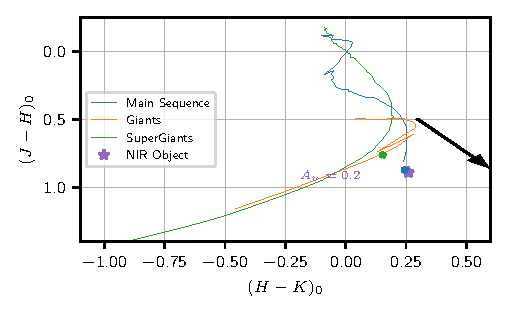
\includegraphics{CodeAndFigures/ASTRO643_HW4P4plot.pdf}
    \caption{Color-Color diagram}
    \label{fig:ColorColorDiagram}
\end{figure}

\Needspace{8\baselineskip}
\subsection{}
\textbf{Assuming that the near-IR object is either a main sequence star or a giant star, estimate or constrain its extinction and compare it with the value inferred from the X-ray absorbing gas column density toward the X-ray source (using the $N_H/A_V = 1.8\times 10^{21} \text{atoms cm}^{-2} \text{ mag}^{-1}$).
Is the near-IR object likely to be the counterpart of the X-ray source?
Similar methods may be used to probe the nature of other types of objects (e.g., galaxies, accounting for extinction and red-shift effects).}

From the column density, we can determine that the extinction of the X-ray is given by 
\begin{equation*}
    A_v = \frac{N_H}{(N_H/A_V)} = \frac{(5\pm0.5)\times10^{22} \si{\per\cm\squared}}{1.8\times 10^{21} \text{ cm}^{-2} \text{ mag}^{-1}} = \num{27.777}\pm2.7 
\end{equation*}

Using different values of extinction, we determined that the needed extinction for the near infrared object to reach:
\begin{itemize}
    \item Main Sequence branch: $A_V=0.45$
    \item Giants branch: $A_V=1.5$
    \item Super Giants branch: $A_V=1.9$
\end{itemize}

All of these values are too small compared to the estimated value of the extinction of the X-ray source. IS for this reason that we determined that the NIR object is not likely to be a counterpart to the X-ray source. 


%==============================================================

\section{}(10 points)
\textbf{Assuming that the star formation rate for the Galaxy is $6 M_\odot \si{\per\year}$ for the last 1 Gyr or so.}
\subsection{} 
\textbf{Please express and plot an appropriately-scaled differential Salpeter initial mass function (IMF) with an index of $x = 2.35$ for $M \geq 0.5M_\odot$ and $x = 1.3$ for
$0.1M_\odot\leq M < 0.5M_\odot$; the IMF should have a continuity at the break point.}

The Salpeter initial mass function will be given by
\begin{equation*}
    IMF = \frac{dn}{dM} = 
    \begin{cases} 
      A(M/M_\odot)^{-1.3}     & 0.1M_\odot < M < 0.1M_\odot\\
      B(M/M_\odot)^{-2.35}    & M \geq 0.5M_\odot
   \end{cases}
\end{equation*}
where A and B are scaling coefficients. 

Given that both equations need to be continuous at $0.5M_\odot$ we can find a relationship between the coefficients by
\begin{equation*}
    A(0.5)^{-1.3}=B(0.5)^{-2.35} \qquad\rightarrow\qquad A = \frac{B(0.5)^{-2.35}}{(0.5)^{-1.3}} = B*0.5^{-1.05}
\end{equation*}

Integrating the IMF from $0.1M_\odot$ to $100M_\odot$ and substituting A, we get
\begin{align*}
    n &= \int_{0.1M_\odot}^{0.5M_\odot}A(M/M_\odot)^{-1.3}dM + \int_{0.5M_\odot}^{100 M_\odot}B(M/M_\odot)^{-2.35}dM 
    =\left[\frac{A(M/M_\odot)^{-0.3}}{-0.3}\right]_{0.1M_\odot}^{0.5M_\odot} + \left[\frac{B(M/M_\odot)^{-1.35}}{-1.35}\right]_{0.5M_\odot}^{100 M_\odot}\\
    &= \frac{A}{-0.3}(0.5^{-0.3}-0.1^{-0.3})+\frac{B}{-1.35}(100^{-1.35}-0.5^{-1.35})
    = 2.5470A + 1.8867B \\
    &= 2.5407(B*0.5^{-1.05}) + 1.8867B = 7.1605B
\end{align*}
So given that n is equal to the star formation rate, we can find that
\begin{align*}
    B = 6 /1.8867 = 0.8379 ,\text{ and}\\
    A = B*0.5^{-1.05} = 1.7349 
\end{align*}

So the final IMF is plotted in Figure \ref{fig:IMF} and is given by
\begin{equation*}
    IMF = \frac{dn}{dM} = 
    \begin{cases} 
      1.7349(M/M_\odot)^{-1.3}     & 0.1M_\odot < M < 0.1M_\odot\\
      0.8379(M/M_\odot)^{-2.35}    & M \geq 0.5M_\odot
   \end{cases}
\end{equation*}

\begin{figure}
    \centering
    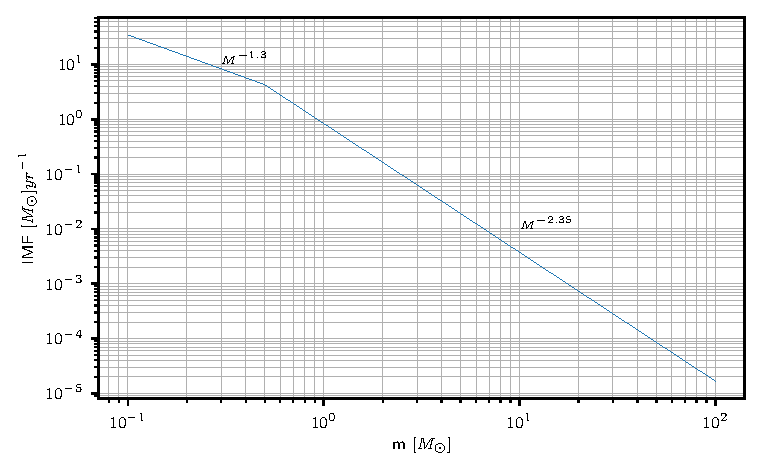
\includegraphics{CodeAndFigures/ASTRO643_HW4P5plot.pdf}
    \caption{Salpeter IMF with index of $x = 2.35$ for $M \geq 0.5M_\odot$ and $x = 1.3$ for $0.1M_\odot\leq M < 0.5M_\odot$ and normalized to $6 M_\odot \si{\per\year}$}
    \label{fig:IMF}
\end{figure}

\Needspace{8\baselineskip}
\subsection{}
\textbf{Further assuming that all stars between $8$ and $100M_\odot$ explode as core-collapsed supernovae, estimate the corresponding present supernova rate. 
How much difference does it make if the upper mass limit for supernovae is assumed to be infinite? (The observed rate for
core-collapsed supernovae in galaxies like our own is of the order of 2 to 3 per century.)}

The supernova rate (SNR) can be derived from the integration of the Initial Mass Function so the supernovas per year are given by,
\begin{align*}
    SNR = \int_{8M_\odot}^{100M_\odot}0.8379(M/M_\odot)^{-2.35} = 0.0362\quad SN yr^{-1} = 3.62 \text{ SN century}^{-1}\\
    SNR = \int_{8M_\odot}^{\infty}0.8379(M/M_\odot)^{-2.35} = 0.0375\quad SN yr^{-1} = 3.75 \text{ SN century}^{-1}\\
\end{align*}

The difference is only $0.13$ supernovas per century. It makes sense since there are a very small number of massive stars than lower massive stars. So the lower massive stars have a higher contribution to the Supernova rate. 

\appendix
\newpage

\section[]{Python code} 
\lstset{caption={Astro643Hw4.py}, style=Python}
\lstinputlisting[language=Python]{CodeAndFigures/Astro643Hw4.py}

